\subsection{Lựa chọn công nghệ}

\subsubsection{Frontend}

\subsubsection*{Mục tiêu}
\begin{itemize}[leftmargin=*]
    \item Cross-platform mobile (Android/iOS)
    \item Hiển thị bản đồ, GPS, cập nhật real-time
    \item Kết nối REST API \& WebSocket
    \item Hiệu năng tốt, UI thân thiện
\end{itemize}

% \subsubsection{So sánh ngôn ngữ phổ biến}

% \begin{table}[h]
% \centering
% \begin{tabular}{>{\bfseries}p{3cm}p{5cm}p{5.5cm}}
% \toprule
% \textbf{Ngôn ngữ} & \textbf{Ưu điểm} & \textbf{Nhược điểm} \\
% \midrule
% Dart (Flutter) & Hiệu năng cao (native code). \newline UI đồng nhất, đẹp. \newline Clean Architecture tự nhiên. \newline Hot reload nhanh. & Không cùng stack với backend. \newline Không tái sử dụng code web. \newline Kích thước APK lớn. \\
% \addlinespace
% JavaScript/TypeScript (React Native) & Cùng ngôn ngữ backend. \newline Tái sử dụng logic web. \newline Cộng đồng lớn. \newline APK nhỏ hơn. & Hiệu năng thấp hơn Flutter. \newline Phụ thuộc bridge JS-Native. \newline UI ít đồng nhất. \\
% \bottomrule
% \end{tabular}
% \end{table}

\subsubsection*{Một số framework front-end phổ biến}

\begin{longtable}{|>{\raggedright\arraybackslash}p{3.5cm}|>{\raggedright\arraybackslash}p{5cm}|>{\raggedright\arraybackslash}p{5cm}|}
\hline
\textbf{Tiêu chí} & \textbf{Flutter (Dart)} & \textbf{React Native (JS/TS)} \\
\hline
\endfirsthead
\hline
\textbf{Tiêu chí} & \textbf{Flutter} & \textbf{React Native} \\
\hline
\endhead
\hline
\endfoot

Hiệu năng & \textbf{Rất cao (native code)} & Tốt (bridge JS-Native) \\
\hline
Tích hợp bản đồ & Google Maps, Mapbox plugin & react-native-maps \\
\hline
Real-time (WebSocket) & socket\_io\_client & Socket.io (cùng stack) \\
\hline
UI customization & \textbf{Rất cao, đồng nhất} & Phụ thuộc native components \\
\hline
Kích thước APK & Lớn hơn (60-80MB) & Nhỏ hơn (40-50MB) \\
\hline
Cộng đồng & Đang phát triển mạnh & Lớn, nhiều thư viện \\
\hline
Clean Architecture & \textbf{Tốt nhất (domain-data-presentation)} & Khả thi (Redux + layers) \\
\hline
Hot reload & \textbf{Rất nhanh} & Nhanh \\
\hline
Learning curve & Cao (Dart mới) & Thấp (JS phổ biến) \\
\hline
Tích hợp backend Node.js & Tốt (REST/WebSocket) & \textbf{Rất tốt (cùng JS)} \\
\hline
Tái sử dụng code web & Không (riêng Flutter Web) & \textbf{Có (React.js)} \\
\hline
\end{longtable}

% \subsubsection{Lựa chọn: Flutter}

\textbf{Lựa chọn Flutter:}
\begin{itemize}[leftmargin=*]
    \item \textbf{Hiệu năng vượt trội}: Compile ra native code, không cần bridge → mượt mà hơn, quan trọng cho ứng dụng bản đồ real-time
    \item \textbf{UI đồng nhất và đẹp}: Widget system mạnh mẽ, giao diện giống hệt trên iOS và Android
    \item \textbf{Clean Architecture tự nhiên}: Dart hỗ trợ tốt pattern domain-data-presentation, dependency injection rõ ràng
    \item \textbf{Hot reload nhanh}: Tăng tốc độ phát triển, debug dễ dàng
    \item \textbf{Phù hợp dự án học tập}: Thể hiện kỹ năng học công nghệ mới, kiến trúc rõ ràng hơn
    \item \textbf{Google hỗ trợ}: Tài liệu tốt, plugin chính thức (Maps, Location, WebSocket)
\end{itemize}

\textbf{Trade-off chấp nhận được:}
\begin{itemize}[leftmargin=*]
    \item Không cùng ngôn ngữ với backend: Vẫn giao tiếp tốt qua REST API và WebSocket, không ảnh hưởng kiến trúc Clean
    \item APK lớn hơn: Chấp nhận được với mobile hiện đại (storage đủ lớn)
    \item Learning curve: Dart dễ học, syntax giống Java/JavaScript
\end{itemize}

\subsubsection{Backend}

\subsubsection*{Mục tiêu}
\begin{itemize}[leftmargin=*]
    \item Tương thích Clean Architecture (Layered)
    \item Hỗ trợ REST API, WebSocket, database
    \item Tích hợp AI module và P2P service
    \item Dễ deploy trên cloud
    \item Dễ mở rộng module (Auth, Payment, AI)
\end{itemize}

\subsubsection*{Lựa chọn ngôn ngữ}

\begin{longtable}{|>{\raggedright\arraybackslash}p{2.5cm}|>{\raggedright\arraybackslash}p{5cm}|>{\raggedright\arraybackslash}p{5.5cm}|}
\hline
\textbf{Ngôn ngữ} & \textbf{Ưu điểm} & \textbf{Nhược điểm / Đánh giá} \\
\hline
\endfirsthead
\hline
\textbf{Ngôn ngữ} & \textbf{Ưu điểm} & \textbf{Nhược điểm / Đánh giá} \\
\hline
\endhead
\hline
\endfoot

Java & Chuẩn doanh nghiệp, DI tốt, bảo mật mạnh & Nặng, setup phức tạp. \newline \textbf{Không phù hợp đồ án.} \\
\hline
JavaScript/ TypeScript (Node.js) & Non-blocking I/O, hiệu năng cao. \newline Hỗ trợ real-time tốt (Socket.io). \newline Dễ tổ chức Clean Architecture. \newline Cùng ngôn ngữ với frontend. & Xử lý logic đồng bộ phức tạp cần cẩn thận. \newline \textbf{Rất phù hợp.} \\
\hline
Python & ORM mạnh (Django), dễ tích hợp AI & WebSocket phức tạp (Channels). \newline Cấu trúc MTV cứng nhắc. \newline \textbf{Phù hợp trung bình.} \\
\hline
\end{longtable}

\textbf{Lựa chọn: JavaScript/TypeScript (Node.js)}
\begin{itemize}[leftmargin=*]
    \item Cùng ngôn ngữ với frontend React Native → chia sẻ types, dễ debug
    \item Non-blocking I/O → phù hợp xử lý nhiều request đồng thời
    \item Hỗ trợ WebSocket tốt → phù hợp P2P và real-time
    \item Dễ gọi AI service Python qua REST API
    \item Cộng đồng lớn, dễ deploy
\end{itemize}

\subsubsection*{Các framework back-end Node.js phổ biến}

\begin{longtable}{|>{\raggedright\arraybackslash}p{2.5cm}|>{\raggedright\arraybackslash}p{5cm}|>{\raggedright\arraybackslash}p{6cm}|}
\hline
\textbf{Framework} & \textbf{Ưu điểm} & \textbf{Nhược điểm / Đánh giá} \\
\hline
\endfirsthead
\hline
\textbf{Framework} & \textbf{Ưu điểm} & \textbf{Nhược điểm / Đánh giá} \\
\hline
\endhead
\hline
\endfoot

Express.js & Nhẹ, linh hoạt, đơn giản & Không có cấu trúc sẵn, cần tự tổ chức. \newline Thiếu DI, decorator. \newline \textbf{Phù hợp dự án nhỏ.} \\
\hline
NestJS & Kiến trúc module rõ ràng. \newline DI, decorator tích hợp sẵn. \newline Hỗ trợ TypeScript tốt. \newline Template Clean Architecture có sẵn. \newline WebSocket built-in. & Phức tạp hơn Express. \newline Learning curve cao hơn. \newline \textbf{Rất phù hợp Clean Architecture.} \\
\hline
Fastify & Hiệu năng cao nhất & Cộng đồng nhỏ hơn. \newline Plugin ít hơn. \newline \textbf{Phù hợp trung bình.} \\
\hline
\end{longtable}

\textbf{Lựa chọn: NestJS}
\begin{itemize}[leftmargin=*]
    \item Hỗ trợ Clean Architecture tốt nhất (module, DI, layers)
    \item Decorator và TypeScript → code rõ ràng, dễ bảo trì
    \item WebSocket tích hợp sẵn → phù hợp P2P và real-time
    \item Template có sẵn cho Clean Architecture
    \item Dễ mở rộng module (Auth, Payment, AI)
\end{itemize}

\textbf{Ngoài ra chọn: Python (FastAPI) cho triển khai AI/ML Service sau này}
\begin{itemize}[leftmargin=*]
    \item Python là ngôn ngữ chuẩn cho ML/AI (scikit-learn, TensorFlow, PyTorch)
    \item FastAPI: hiệu năng cao, async, dễ tích hợp model
    \item Chạy độc lập như microservice, giao tiếp với backend qua REST API
    \item Không ảnh hưởng đến kiến trúc chính
\end{itemize}

\subsubsection{Database}
\subsubsection*{Mục tiêu}
\begin{itemize}[leftmargin=*]
    \item Lưu trữ dữ liệu quan hệ (users, vehicles, rentals, payments)
    \item Hỗ trợ transaction (ACID) cho payment và booking
    \item Hiệu năng tốt cho truy vấn phức tạp (join, aggregation)
    \item Khả năng mở rộng và backup dễ dàng
    \item Tích hợp tốt với NestJS (ORM)
\end{itemize}
\textbf{Lựa chọn PostgreSQL:}
\begin{itemize}[leftmargin=*]
    \item \textbf{ACID compliance}: Đảm bảo tính toàn vẹn dữ liệu cho payment và rental transactions
    \item \textbf{Spatial data support}: PostGIS extension hỗ trợ location queries (tìm xe gần, tính khoảng cách)
    \item \textbf{JSON support}: Lưu trữ metadata linh hoạt (vehicle specifications, user preferences)
    \item \textbf{TypeORM integration}: NestJS tích hợp sẵn TypeORM, hỗ trợ PostgreSQL tốt nhất
    \item \textbf{Advanced features}: Full-text search, materialized views, trigger cho event-driven
    \item \textbf{Scalability}: Replication, partitioning cho mở rộng sau này
    \item \textbf{Open-source}: Không phí license, cộng đồng lớn
\end{itemize}
% \subsubsection*{Một số cơ sở dữ liệu phổ biến}

% \begin{longtable}{|>{\raggedright\arraybackslash}p{2.5cm}|>{\raggedright\arraybackslash}p{5cm}|>{\raggedright\arraybackslash}p{6cm}|}
% \hline
% \textbf{Database} & \textbf{Ưu điểm} & \textbf{Nhược điểm / Đánh giá} \\
% \hline
% \endfirsthead
% \hline
% \textbf{Database} & \textbf{Ưu điểm} & \textbf{Nhược điểm / Đánh giá} \\
% \hline
% \endhead
% \hline
% \endfoot

% PostgreSQL & ACID compliance mạnh. \newline Hỗ trợ JSON, spatial data (PostGIS). \newline TypeORM tích hợp tốt với NestJS. \newline Open-source, cộng đồng lớn. \newline Hỗ trợ index, full-text search. & Setup phức tạp hơn MySQL. \newline \textbf{Rất phù hợp cho dữ liệu quan hệ + location.} \\
% \hline

% MySQL & Phổ biến, dễ setup. \newline Hiệu năng tốt cho read-heavy. \newline Cộng đồng lớn. & Không mạnh về JSON và spatial queries. \newline Ít tính năng nâng cao hơn PostgreSQL. \newline \textbf{Phù hợp trung bình.} \\
% \hline

% MongoDB & Linh hoạt schema (NoSQL). \newline Tốt cho dữ liệu phi cấu trúc. & Không ACID mặc định. \newline Không phù hợp dữ liệu quan hệ phức tạp. \newline \textbf{Không phù hợp làm DB chính.} \\
% \hline
% \end{longtable}



% \subsection{Cache \& Message Queue}

% \subsubsection{Redis - Multi-purpose}

% \textbf{Vai trò:}
% \begin{itemize}[leftmargin=*]
%     \item \textbf{Cache layer}: Cache API response, session data, frequently accessed data
%     \item \textbf{Session store}: Lưu JWT tokens, user sessions
%     \item \textbf{Pub/Sub}: Message queue cho event-driven architecture
%     \item \textbf{Real-time data}: Lưu vị trí xe real-time (geospatial data)
%     \item \textbf{Rate limiting}: Giới hạn API requests
% \end{itemize}

% \textbf{Use cases cụ thể:}
% \begin{table}[h]
% \centering
% \small
% \begin{tabular}{>{\bfseries}p{4cm}p{9.5cm}}
% \toprule
% \textbf{Feature} & \textbf{Cách sử dụng Redis} \\
% \midrule
% Session Management & Key: \texttt{session:\{userId\}}, Value: JWT token + metadata, TTL: 7 days \\
% \addlinespace
% Vehicle Location Cache & Sorted Set: \texttt{vehicles:location}, Score: timestamp, Member: vehicleId + lat/lng \\
% \addlinespace
% Event-driven & Pub/Sub channels: \texttt{rental:started}, \texttt{vehicle:updated}, \texttt{payment:completed} \\
% \addlinespace
% API Cache & Key: \texttt{api:\{endpoint\}:\{params\}}, TTL: 5-60 minutes \\
% \addlinespace
% Rate Limiting & Key: \texttt{ratelimit:\{userId\}:\{endpoint\}}, Increment + TTL: 1 minute \\
% \bottomrule
% \end{tabular}
% \end{table}
\subsection{Sơ đồ triển khai hệ thống}
\begin{figure}[H]
    \centering
    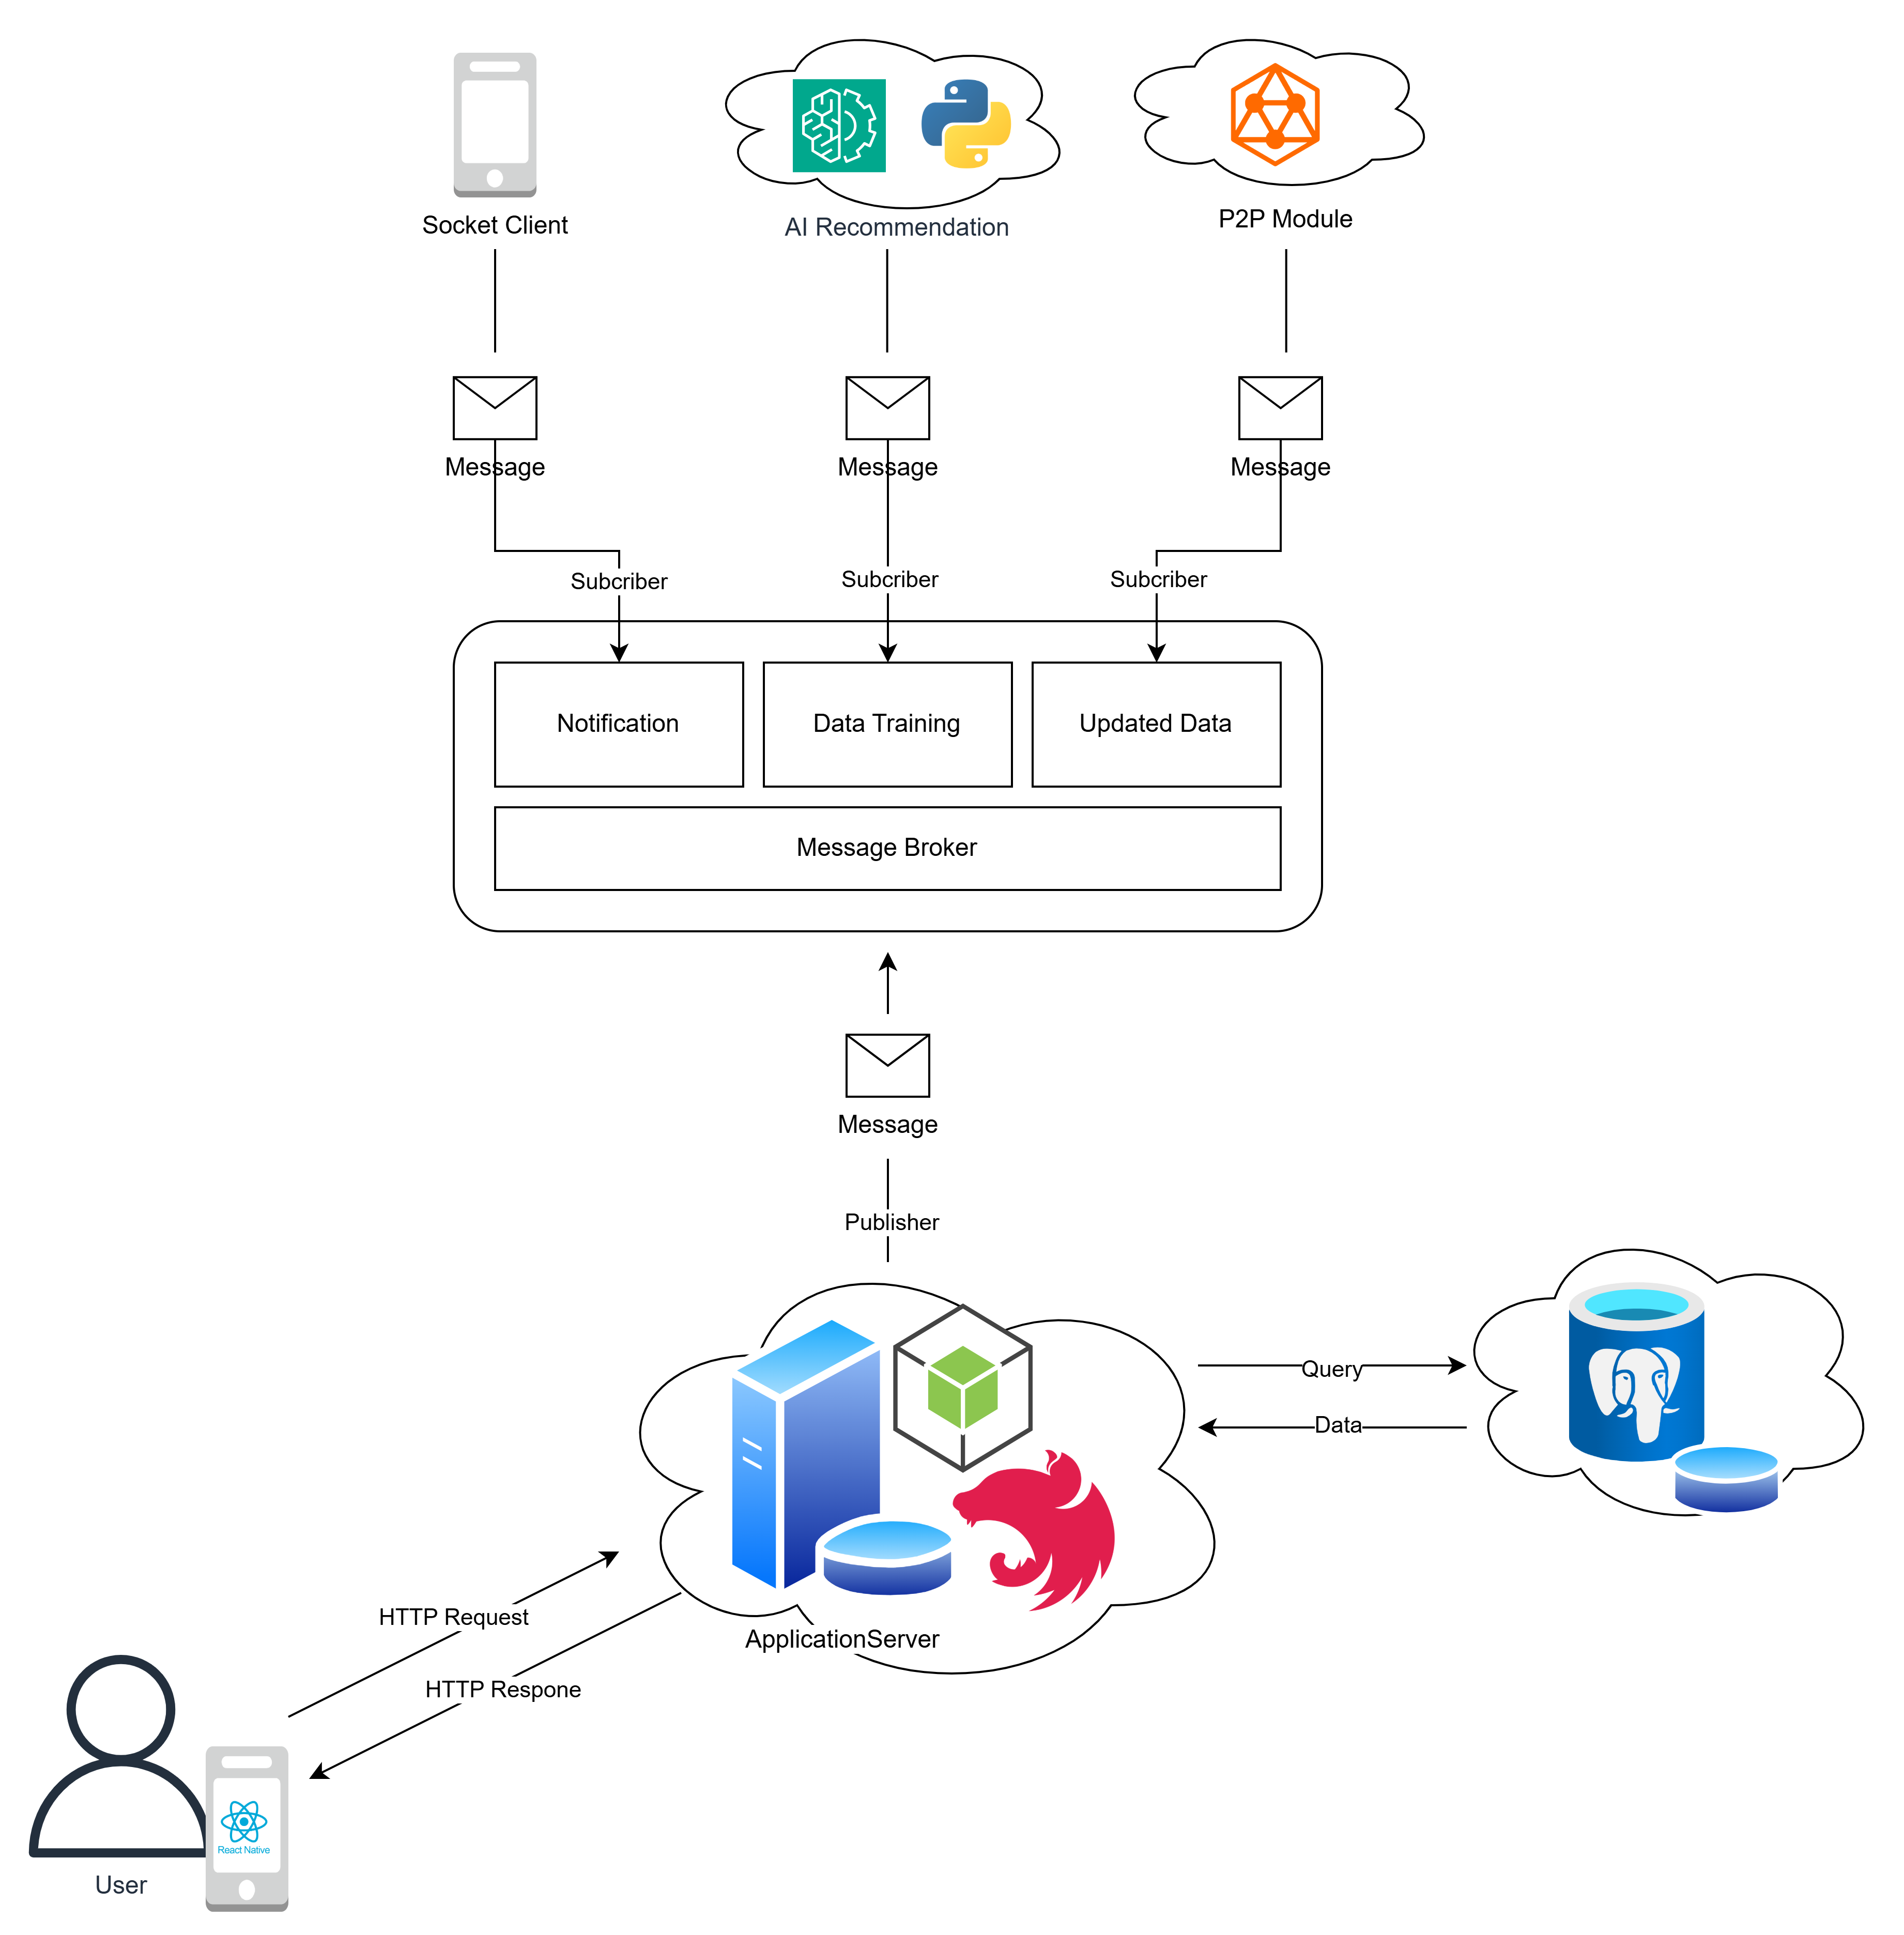
\includegraphics[width=0.7\textwidth]{Images/Deploy/arch.png}
    \caption{Deployment Diagram}
    \label{fig:deployment-diagram}
\end{figure}